\chapter{Literature Review}
\label{ch:litreview}

This review broadly categorises the effects of \ac{LCC} on \ac{SW} into those resulting from vegetation cover change and those resulting from urbanisation, then examines these separately in the following subsections. The two cannot be completely dissociated since a loss of vegetation cover usually accompanies urbanisation. But a rough distinction can be made in that the latter pertains to effects particular to urban development that are not necessarily applicable to other \ac{LCC} types and which is mainly described in terms of thermal and mechanical characteristics, while the former pertains to effects which can be attributed to changes in natural characteristics (which may be present even without urbanisation as in the case of vegetation loss) and incorporates biospheric feedback mechanisms.

\section[Methods for analysing land cover change]{Methodologies for analysing the effect of land cover change}

In a review of recent progress in \ac{NSWS} change research in China \citep{zha2021}, broadly categorised studies on the effect of \ac{LCC} into \ac{UMR}, \ac{OMR} and \acp{FWM}. \ac{UMR} examines the difference between observational data from urban and rural weather stations. As it uses direct observations, results have higher fidelity than modelled results, but is particularly weak for regions where there is a lack of data (mainly rural areas and developing countries). \ac{OMR} compares observational data against reanalysis with inputs simulating unchanged land cover. \ac{OMR} methods can be used up to a global scale but the data can have model-introduced artefacts, especially at smaller spatial scales due to the coarse resolution of \acp{GCM} \citep{zha2021}. \acp{FWM} quantify effects based on simple dynamic models, but it ignores important effects such as turbulent flux, horizontal advection, temporal changes in horizontal winds, and is also difficult to use in complex terrain \citep{zha2021}.

\section{Datasets and models}

Studies have been complicated by the sparsity of \ac{AWS} data (especially in rural areas and developing countries), as well as biases present in reanalysis datasets. Reanalysis datasets often overestimate \acp{SWS} \citep{fan2021}, and there is an especially large disparity for \acp{DMWS} \citep{zhang2020, zhang2022}. \citet{zhang2019} found that \acp{SWS} from the \ac{JRA55} reanalysis dataset had the closest agreement with observations in China, but \citet{ramon2019} noted that this dataset has unusually high interannual variability, and that \ac{ERA5} instead offers the best agreement with observational wind speeds and interannual variability on a global scale. The latter is consistent with analysis by \citet{torralba2017} which found that \ac{JRA55} displayed intensified trends.

\section[Recent trends in near-surface wind speed]{Observed changes in near-surface wind speed over the last few decades}

\subsection{Slowdown and "global terrestrial stilling"}

Much of the recent research regarding the effect of \ac{LCC} on \ac{SW} has been under the context of a global decline in \ac{NSWS} observed in recent decades, a phenomenon which has come to be known as “global terrestrial stilling”. \ac{LCC} was heavily implicated as a cause for this \ac{NSWS} decline, but recent analyses such as \citep{zeng2019} have identified a reversal in this decline at different periods for various continents, which along with other other evidence such as historical multidecadal declines found in centennial-scale reanalysis \citep{shen2021}, suggests that large-scale oscillations in atmospheric circulations may be at play.

Most existing studies on \ac{LCC}-\ac{NSWS} interactions have been on the various regions of China, perhaps because of the country’s rapid urbanisation eliciting stronger wind responses in recent decades coinciding with the rise of \ac{AWS} \ac{NSWS} measurements, and because of close monitoring accompanying large-scale afforestation efforts to combat wind erosion. Focus studies on regions outside of China have occasionally been conducted (summarised in Table~\ref{tab:nsws}), but these have yielded limited insights beyond what has already been learned in China. However, there has been a wealth of research on the climatic effects of \ac{LCC} more generally and these often yield additional information into \ac{SW} changes. A challenge in research has been to dissociate these changes and quantify the component which is due to \ac{LCC}.

\begin{table}\centering
	\ra{1.3}
	\caption[Summary of surface wind speed trends in global literature]{A summary of research specifically studying \ac{SWS} changes in a region outside of China (non-exhaustive).}
	\label{tab:nsws}	
	\begin{tabular}{@{}p{8.5cm}p{2.5cm}p{2cm}@{}}
		\toprule
		\textbf{Country (Study)} & \textbf{Time Period} & \textbf{Wind speed change (m/s/yr)} \\ \midrule
		Australia \citep{mcvicar2008} & 1975-2006 & -0.009 \\ \midrule
		India \citep{jaswal2013} & 1961-2008 & -0.024 \\ \midrule
		Portugal and Spain \citep{azorin-molina2014} & 1961-2011 & -0.0016 \\
		& 1979-2008 & -0.001 \\ \midrule
		Sweden \citep{minola2016, minola2022} & 1956-2013 & -0.006 \\
		& 1979-2008 & -0.001 \\
		& 1997-2003 & -0.044 \\
		& 2003-2019 & -0.004 \\ \midrule
		Saudia Arabia \citep{azorin-molina2018} & 1978-2001 & -0.0089 \\
		& 2001-2003 & +0.0057 \\
		\bottomrule
	\end{tabular}
\end{table}

%\newcolumntype{P}[1]{>{\centering\arraybackslash}p{#1}}
%\begin{center}
%	\begingroup
%	\renewcommand\arraystretch{0.66} % only applicable to this table because of group
%	
%	\begin{longtable}{P{6cm}P{4cm}P{3cm}}
	%		\caption[Summary of surface wind speed trends in global literature]{A summary of research specifically studying \ac{SWS} changes in a region outside of China (non-exhaustive).} 
	%		\label{tab:nsws} 
	%		\\ 
	%		\toprule 
	%		\multicolumn{1}{P{6cm}}{\textbf{Country (Study)}}
	%		& \multicolumn{1}{P{4cm}}{\textbf{Time Period}}
	%		& \multicolumn{1}{P{3cm}}{\textbf{Wind speed change (m/s/yr)}}\\	
	%		\midrule
	%		\endfirsthead
	%		\midrule
	%		\multicolumn{1}{P{6cm}}{\textbf{Country (Study)}}
	%		& \multicolumn{1}{P{4cm}}{\textbf{Time Period}}
	%		& \multicolumn{1}{P{3cm}}{\textbf{Wind speed change (m/s/yr)}}\\	
	%		\midrule	
	%		\endhead
	%		\midrule	
	%		\multicolumn{3}{l@{}}{(continued\ldots)}\\
	%		\endfoot
	%		\endlastfoot
	%		Australia \citep{mcvicar2008} & 1975-2006 & -0.009 \\ \midrule
	%		India \citep{jaswal2013} & 1961-2008 & -0.024 \\ \midrule
	%		Portugal and Spain \citep{azorin-molina2014} & 1961-2011 & -0.0016 \\
	%		 & 1979-2008 & -0.001 \\ \midrule
	%		Sweden \citep{minola2016, minola2022} & 1956-2013 & -0.006 \\
	%		 & 1979-2008 & -0.001 \\
	%		 & 1997-2003 & -0.044 \\
	%		 & 2003-2019 & -0.004 \\ \midrule
	%		Saudia Arabia \citep{azorin-molina2018} & 1978-2001 & -0.0089 \\
	%		 & 2001-2003 & +0.0057 \\
	%		\bottomrule
	%	\end{longtable}
%	
%	\endgroup
%\end{center}

Using weather station observations from 1960 to 1999, \citet{li2008} found that \ac{NSWS} in China decreased by 0.013 m/s/yr from 1960 to 1968, 0.023 m/s/year from 1969 to 1991 and 0.003 m/s/yr from 1991 to 1999 (punctured by changes in measurement instruments around 1970). Furthermore, the authors analysed the effect of \ac{LCC} using the \ac{OMR} method but with reanalysis data where surface observations of temperature, moisture and wind were omitted. They found that \ac{NSWS} had a declining decadal trend north of Shandong irrespective of \ac{LCC}, but that the exclusion of \ac{LCC} south of Shandong resulted in an increasing trend instead. However, the methodology of excluding surface observations from reanalysis data to simulate natural land cover is controversial since it might not capture crucial surface properties, and rural weather station data availability was relatively sparse. Subsequent studies have then sought to quantify effects on a more nuanced basis such as by comparing between cities of different sizes and urbanisation rates (discussed later).

\subsection{Results confounded by instrument drift}

It is important to note that part of these declines may in part be due to measurement drift in ageing anemometers. A study by \citet{azorin-molina2018_drift} compared new and old SEAC SV5 anemometers (the dominant anemometer model used by the Spanish Meteorological Agency since the mid-1980s), and found median biases of around 0.3 m/s. Assuming a linear drift over 30 years this could constitute around 0.01 m/s/year of wind speed changes (on the order of the observed declines), but results need to be interpreted carefully since not all studies made bias corrections and other regions use different anemometer models which are subject to different weather conditions. Furthermore, such drifts do not necessarily invalidate the attributed effects of \ac{LCC} and large-scale atmospheric oscillations since observations on the geospatial variability of \ac{NSWS} changes still implicate these factors (discussed in later subsections).

\section{The effect of urbanisation}

\subsection{Urban minus Rural}

\citet{guo2011} found similar decreases in \ac{NSWS} (0.025 m/s/yr from 1969 to 1990 and 0.006 m/s/yr from 1990 to 2005) as \citet{li2008}, and furthermore divided the results between urban and rural weather stations. The authors found a comparable rate of decrease between urban and rural from 1969 to 1990, a cotemporaneous decrease in the 850 hPa pressure-gradient force within the region from reanalysis data, and that much of this decline manifested in weaker strong wind events - the former two points suggesting that weakening winds were associated with large-scale atmospheric circulations.

\subsection{Wind speed anomalies}

\citet{guo2011} also discovered a temporary increase in urban wind speeds from 1990 to 1995 while rural winds were still decreasing, in spite of the fact that peaking Chinese urbanisation in the late 1980s to early 1990s would have increased urban frictional drag. The authors cited a similar discovery in southeast Queensland and northeast New South Wales, Australia by \citet{mcvicar2008} and suggested the effect for further investigation. It’s not clear whether there is a causal relationship between urbanisation and the wind speed increase, but a regional-scale urban Venturi effect is one possible explanation (although this would require further examination).

The wind increase from 1990 to 1995 could also be associated with enhanced turbulence mixing in momentum from a deepened \ac{ABL} and interactions with geostrophic accelerations, in what \citet{droste2018} called an \acf{UWI} effect. \citet{droste2018} conducted simulations using a surface model with different urban local climate zones, along with a conceptual bulk model with idealised assumptions representing the mixed layer. The results showed that contrary to standard assumptions, “the mean wind in cities can exceed the wind in the rural surrounding”, and that this \ac{UWI} enhancement occurs primarily during daytime with a typical early afternoon peak of 0.5 ms-1.

\subsection{Extreme winds}

Urbanisation may also influence the occurrence of extreme wind events. Results by \citet{zhang2020, zhang2022} show a decline in \ac{DMWS} in areas of China, with the highest declines observed in regions with high urbanisation rates. Furthermore, the decline was found in observational data but not reanalysis datasets such as NCEP-NCAR1 and \ac{ERA5}, suggesting that changes are more likely a result of urbanisation than atmospheric circulation changes.

Furthermore, earlier analysis by \citet{gero2006} studied the effects of \ac{LCC} on storms in the Sydney Basin, Australia using numerical modelling simulations. The authors found little effect on frontal storms, greater horizontal accelerations over smooth agricultural land during convective storms, and that “in a special case, the dense urban surface of Sydney’s city core appears to trigger an intensive convective storm.” However, it isn’t clear whether this manifests as an increased prevalence in storms and extreme wind events, nor whether this has been observed in other regions.

\subsection{Rate of urbanisation and size of cities}

Building on previous work by \citet{guo2011}, \citet{zha2017} further examined the difference in China’s \ac{NSWS} declines between large and small cities. The authors found that the urbanisation rate of a city was positively correlated with greater \ac{NSWS} declines, with a 10\% higher urbanisation rate roughly associated with a 0.11 m/s faster decline. By first correcting for systematic errors then applying the \ac{OMR} method, the authors found that the \ac{LCC} could account for decreases of 0.057 m/s/yr and 0.030 m/s/yr in large and small cities respectively (despite large cities having a lower mean \ac{NSWS} to begin with). The authors noted that comparisons were confounded by geographically uneven development and so studied adjacent large-small city pairs using the \ac{UMR} method, again finding that \ac{LCC} effects on large cities were more significant, but also that accounting for geographical uneven development in this way produced closer agreement with the \ac{OMR} method. Interestingly, the authors found that the phase of annual and seasonal \ac{NSWS} cycles were the same across both large and small cities - evidence that \ac{NSWS} changes are not due to urbanisation alone but also large-scale atmospheric circulation changes.

In similar studies by the same authors, \citet{zha2016, zha2017_zones} divided up the results into 6 different wind speed categories and 4 climate zones, finding that urbanisation narrowed the \ac{NSWS} probability distribution and led to a stronger decline in strong wind categories, consistent with earlier discoveries by \citet{guo2011}. Furthermore, it was found that the \ac{NSWS} probability distribution of similar-sized cities were different across climate zones, again suggesting that a holistic account of \ac{NSWS} changes needs to incorporate both the effect of \ac{LCC} and regional climate change.

\subsection{Urban heating}

\citet{guo2011} also noted that temperature increases from urbanisation may affect the pressure-gradient force so that declining winds cannot be attributed to large-scale circulations alone, and indeed later analysis by \citet{zhang2021} suggests a likely contribution from uneven heating. This is also consistent with earlier findings by \citet{kitada1998}, who conducted simulations using a mesoscale meteorological model and found that urban heating effects in the Nohbi Plain of central Japan established a pressure-gradient force adverse to topographically induced winds, resulting in a weak wind zone downwind of the urban area. Urban areas can also delay sea breezes through their drag effect, as was confirmed in numerical simulations by \citet{rajeswari2022}.

Simulation results for the Beijing-Tianjin-Hebei Region by \citet{wang2020} using the \ac{OMR} method in addition show a strong geospatial correlation between \ac{LCC} and subsequently reduced \ac{NSWS}. The results also showed seasonally-dependent modifications of mountain/valley and land/sea breezes, and that the magnitude of \ac{NSWS} decline from urbanisation was relatively low during daytime. The last point is particularly interesting because analysis using observational data by \citet{yu2009} found that wind speeds in this region and beyond are typically much higher during daytime, so when considered as a percentage of the mean wind speed the daytime \ac{NSWS} decline relative to nighttime is even more dramatic. However, it is not clear what causes this effect.

\subsection{Summary}

In summary, there is convincing evidence that the global decrease in \ac{NSWS} over the last few decades was strongly associated with regional-scale atmospheric circulations. The slowing down then subsequent reversal of global stilling is indicative of a cyclical dynamic, and similar periods have appeared in centennial-scale studies. Furthermore, regional-scale 850 hPa pressure-gradients were found to decline during this time, there was a comparable magnitude in wind speed decreases between rural and urban areas during the recent stilling period, annual and seasonal cycles between large and small cities had the same phase, and similar sized cities had different probability distribution changes according to climate zone.

However, attempts to dissociate from this the effect of \ac{LCC} have also found strong evidence that urbanisation had at least localised contributions. Several studies have found a positive correlation between magnitude of wind speed decrease and rate of urbanisation as well as city size. Aside from \ac{NSWS} decline, urbanisation clearly also changes the SW resource in terms of local circulation patterns. Urban areas have seen changing convergence regions, wind speed increase anomalies and weakening of the pressure-gradient force. Modelling further suggests the possibility of wind speed enhancement within an urban area (\ac{UWI} effect), compensatory increases in its periphery, and changes in extreme wind patterns - all of which require further research.

\section[Vegetation-atmosphere interactions]{Vegetation-atmosphere interactions and the effect of agricultural expansion}

\subsection{Roughness length changes}

Vegetation has the obvious effect of increasing surface roughness and hence imparting frictional drag upon \ac{SW}. Afforestation efforts in China were in part deliberately targeting reduced local wind speeds in order to combat wind erosion, with research finding that vegetation cover of at least 10\% was necessary to reduce wind speeds \citep{jiang2019}. In contrast with urban constructions, mechanical characteristics in vegetation cover display more pronounced seasonal characteristics. For example, using an old oak stand in a forested area in Schweinfurt, Germany, \citet{geiger1950} found that although wind speeds below the tree crowns decreased upon leafing, wind speeds above the crown saw a significant increase - possibly a manifestation of the Venturi effect.

Mesoscale modelling studies have also suggested that large-scale deforestation in Australia over the last 200 years has significantly changed near-surface wind patterns and that some of these effects have even been vertically propagated \citep{narisma2003}. In the case of southwest Western Australia, similar modelling by the same authors has suggested increased horizontal wind speeds (owing to reduced roughness length) and decreased vertical velocities in areas with \ac{LCC}, but increased vertical velocities inland of these areas associated with changes in where winds converge \citep{pitman2004}.

\subsection{Surface temperature, pressure and energy balance}

\subsubsection{The Bunny Fence Experiments}

An interesting experimental study was conducted by \citet{nair2011} around the rabbit-proof fence in southwest Australia which sharply delineates native vegetation cover on the eastern side from agricultural land on the western side. The authors used a mix of \ac{OMR} methods, regional atmosopheric numerical modelling, aircraft observations and 3-hourly paired radiosonde releases (20 km east and west of the fence) to examine meteorological differences between vegetation cover types within the summertime and wintertime west coast trough of Australia.

The results show significantly deeper convective development over native vegetation associated with increased cloud cover and a deeper \ac{ABL} (to heights greater than the lifted condensation level). The results also show that a lower mean sea level pressure would be present on the western side of the fence had it still been native vegetation instead of agricultural land, that surface convergence would have occurred closer to this lower pressure region, and that wind field anomalies correlate well with anomalies in \ac{ABL} height, precipitation and surface convergence. This is consistent with simultaneous radiosonde and modelling studies in the Amazon rainforest by \citet{wang2009, xu2022}, who found lower and more shallow cloud cover over deforested areas also associated with \ac{ABL} height changes. 

Interestingly, the results by \citet{nair2011} also show that latent heat fluxes above native vegetation do not vary substantially between summer and winter (unlike agricultural vegetation), suggesting a controlled regime with biophysically damped changes in evapotranspiration and subsequent condensation above native vegetation. Such effects are important since convective developments often drive \ac{SW}, while the \ac{ABL} height affects among other things the vertical wind shear and presence of low-level jets, and understanding of the latter’s effect on winds has in fact been identified as an area of increasing importance for the wind energy and meteorological communities \citep{pena2013}.

Earlier results in the Bunny Fence Experiment series include contributions by \citet{lyons1993, lyons1996, lyons2001, lyons2002, ray2003}, with the dramatic delineation in atmospheric conditions best illustrated in Figure~\ref{fig:cloud_satellite}.

\begin{figure}[!ht]
	\centering
	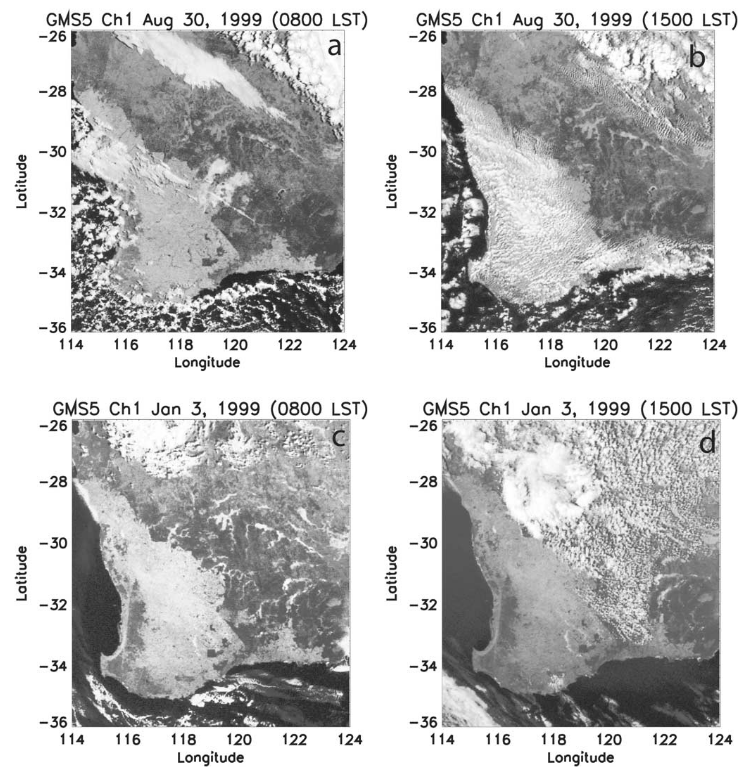
\includegraphics[width=0.75\textwidth]{cloud_satellite.png}
	\caption[Satellite image of delineated cumulus development along fence]{"Preferential development of cumulus clouds in Southwest Australia. (a and b) The preferential development of cumulus clouds over agricultural areas from 0800 to 1500 LT during the winter agricultural season. (c and d) The preferential development of cumulus clouds over native vegetation from 0800 to 1500 LT during the summer dry season." Image and caption copied directly from \citet{ray2003}.}
	\label{fig:cloud_satellite}
\end{figure}

\subsubsection{Mesoscale circulations and vegetation breezes}

There are even internal inhomogeneities within contiguous regions under a single land cover classification. In studying Yatir Forest, Israel, \citet{kroniger2018} found that older and denser growth regions had higher temperatures and produced stronger updrafts for weakly and strongly convective scenarios, pushing up the ABL height and establishing a low pressure area leeward from the older growth at half the ABL height. Being a planted pine forest in an arid region, Yatir Forest had lower albedo, higher net radiation and twice the sensible heat flux (latent flux was negligible in this arid area) compared to the surrounding shrubland. Thermal convections were stronger over the forests (particularly over the older growth areas) which in turn triggered secondary circulations which were coupled with the surrounding shrubland.

A comprehensive review of research on the biogeophysical aspects of \ac{LCC}-climate interactions by \citet{mahmood2014} also concluded that “biogeophysical impacts of \ac{LCC} on local and regional-scale are significant, undeniable and discernible.” On effects pertaining to the wind resource, the authors noted discoveries such as convective clouds developing first over moister vegetated surfaces then secondly over neighbouring dry wheat in humid weather but the converse for a dry atmosphere, increased probability of dust devil formation over cleared agricultural land, and the presence of mesoscale circulations where there is a gradient or abrupt transition in vegetation cover.

The last point is consistent with work by \citet{hong1995, zhuojia1995} using mesoscale biophysical, meteorological models. The results suggested the presence of vegetation breezes at the interface between well irrigated crops and bare soil, arising from a horizontal pressure gradient which is established by uneven surface heating and turbulent mixing in the atmosphere forcing the relatively cold and humid air produced near the canopy by evapotranspiration.

A mesoscale modelling study by \citet{mahmood2011} in Western Kentucky, USA similarly found mesoscale circulations along land cover discontinuities and increased \ac{ABL} height over forest cover. Interestingly, in a comparison between existing land cover and increased forest cover, the results also suggested in the latter case the presence of increased vertical wind speeds and horizontal velocities towards the regions of increased forest cover (convergence) - again suggesting a relationship between vegetation cover and distant advection.

\subsubsection{Temperature and winds}

Observations over a 5-year period by \citet{lapworth2003} at a flat rural inland surface on arable land in Bedfordshire, England found a linear relationship between \ac{NSWS} during evening cooling and screen temperature measured relative to the evening transition. A follow-up study then found that this linear relationship also held for morning heating and that the slope of this relationship showed little change with heating rate, suggesting that \ac{NSWS} during boundary layer transitions were in quasi-equilibrium with temperature (i.e.\ there was little evidence for temperature-independent temporal fluctuations) \citep{lapworth2006}.

\citet{he2013} analysed wind and temperature from 2007 to 2011 at heights of 10, 20, 40, 80, 140 and 200 m using observational data from a meteorological mast in Cabauw, Netherlands (situated in open, flat pastureland). The authors compared the wind speed probability distributions between clear-sky and low-cloud conditions for daytime and nighttime (as determined using a simple algorithm on ceilometer data). The results show a reduced vertical gradient in potential temperature and wind speed during daytime hours, especially for clear-sky conditions - evidence of momentum mixing by thermally-driven turbulence. However, these focus studies were all on flat rural cropland and it’s not clear whether these results hold for other types of land cover.

\subsection{Condensation-induced atmospheric dynamics}
\label{ssec:lit_ciad}

\subsubsection{Theory}

\paragraph{Condensational force, power and pressure gradient}

In a series of papers, \citet{makarieva2009} derived from fundamental thermodynamics principles the existence of what they termed an "evaporative-condensational force" \citep{makarieva2010} with associated "condensational power" \citep{makarieva2014}, and applied this over natural forests (where there is huge amounts of evapotranspiration sustaining this proposed mechanism) to suggest that this is a major driver of atmospheric circulations \citep{makarieva2013}.

This theory holds that upon atmospheric condensation (when the mass density of $H_20$ shrinks upwards of a thousandfold), there is an associated drop in the partial pressure of water vapour and hence pressure of air in general. Local to the point of condensation is an ascension of air from the upwards directed evaporative-condensational force. Over large-scales, this manifests as a horizontal pressure gradient, sustained by condensational power, which affects or gives rise to atmospheric circulations.

\paragraph{The Biotic Pump}

The authors further theorise that forests play an active role in maintaining a higher rate of atmospheric condensation above land than sea (through evapotranspiration from high leaf surface area), so as to advect oceanic moisture inland to replace gravity-induced runoff, in what is known as the "Biotic Pump" \citep{makarieva2009_evidence, makarieva2013_revisiting}. On top of sound (personal judgement) theoretical physics, \citet{makarieva2009_evidence, makarieva2013_revisiting} propose as empirical evidence a set of coast-to-inland transects which demonstrates a sudden increase in precipitation (implicit increase in atmospheric and moisture convergence) from ocean to coast which then remains relatively uniform with inland distance over intact forests. 

The results also show a seasonality which corresponds with forest activity: the Amazon which is active year round controls annual precipitation with tamed season variability, while the Eurasian forest displays precipitation which is greater than that over ocean and is uniform with inland distance only during boreal summer \citep{makarieva2013_revisiting}. The seasonal variability in the latter is especially distinct, with terrestrial precipitation which is not only lower than that over ocean in winter, but which also decreases exponentially with inland distance \citep{makarieva2013_revisiting}. Meanwhile, degraded or unforested areas such as Australia display a year-round precipitation which is less than over ocean and which undergoes exponential decay with distance, with minimal seasonality\citep{makarieva2009_evidence, makarieva2013_revisiting}.

\paragraph{Controversy}

This theory has attracted controversy in part because it goes against the standard view that atmospheric circulations are driven primarily by temperature gradients. In this picture, warmer air rises and leaves behind a low pressure region at the surface, the rising air eventually sinks to create a high pressure region at a neighbouring surface, then surface winds flow from high to low surface pressure. Although it is well-established that this effect exists, theoretical models predict wind energies which fall short by an order of magnitude compared with observations for planetary-scale circulations such as the Hadley cell \citep{held1980, schneider2006, caballero2008, makarieva2013}, down to toy-scale circulations in a purpose-built enclosure specifically investigating this effect \citep{bunyard2015, bunyard2017, bunyard2019}.

Criticisms have also been formulated on physical grounds regarding whether the evaporative-condesational force is theoretically sound\footnote{See exchanges between \citet{meesters2009} and \citet{makarieva2009_meesters}, as well as between \citet{jaramillo2018, jaramillo2019} and \citet{makarieva2019_jaramillo}.}, one of these being that condensation should induce isotropic net flows which cancel each other out \citep{bunyard2015, bunyard2017}. However, a series of experiments by \citet{bunyard2015, bunyard2017, bunyard2019} convincingly demonstrates that anisotropic flow is possible, and anistropic flow from cloud formation is in fact regularly targeted by paragliders for additional lift \citep{pagen1992, pagen2001} (see Section~\ref{sssec:paraglide}). Furthermore, there are good heuristical justifications for why anisotropic flow should result (see Appendix~\ref{sec:anis_cond}).

\subsubsection{Observational evidence by paragliding community}
\label{sssec:paraglide}

Unpowered aircraft enthusiasts have long noted strong lift forces due to condensation near cloud base in a phenomenon known as “cloud suck” \citep{gadd_thermals, pagen1992, pagen2001}, with close-up video evidence also showing a thinned column at the point of condensation resulting from horizontal air advection \citep{benz2021_read}. Also striking is the observation that rising air parcels generating lift exist even on overcast days with little surface heating, with greater prevalence at higher altitudes \citep{rejmanek2018, benz2021_full}. Given that latent heat release occurs above cloud base, and in light of work by \citet{gordon2003, jiang2013, yan2013, zhang2016} strongly suggesting a causal relationship from vegetation cover to water vapour availability via evapotranspiration, vapour pressure drops from condensation may play a mediating role between vegetation cover and long-range advection as suggested in theoretical work by \citet{makarieva2013}.

\subsubsection{Satellite observations display preferential atmospheric convergence over \textit{current} forest cover}

Results from the transect studies by \citet{makarieva2009_evidence, makarieva2013_revisiting} are corroborated by satellite video feeds from \citet{eumetstat}. Video from \citet{eumetstat} shows that terrestrial cloud formation occurs almost exclusively over \textit{current} forest cover. If forest growth was just a passive byproduct of geophysical forces with little influence from forest cover, then there is no reason why clouds shouldn't also form over areas cleared by human activity over recent centuries. So even if forest cover does not actively regulate atmospheric convergence, evidence points towards a modulating effect.

Careful inspection of video from \citet{eumetstat} also reveals a regular diurnal cycle in cloud cover over forests, typically peaking around the evening \ac{ABL} transition. There is also marked seasonality in this cloud cover for forests outside of the tropics.

\subsubsection{Reanalysis of water vapour flows}

\citep{li2020} found that increased vegetation induced a strengthening of winds favourable for water vapour transport towards South China, slow the eastward progression of Rossby waves, and that “In addition to local cooling effects, spring greening was found to cause a decrease in geopotential height … which exerts a significant influence on Ta [surface air temperature] in the Arctic via atmospheric teleconnections … pressure gradients between the Arctic and China are reduced proportionately, resulting in a reduction in the strength of the westerlies over Mongolia.” Interestingly, the authors also found that “Biophysical feedback from atmospheric circulation only emerge over Southeast China, where total cloud cover increases”, and in supplementary figures 5 to 8 present a series of graphs where higher wind speed changes appear to have a geospatial correlation with higher changes in latent energy, humidity and \ac{PW}. These results together suggest that biospherically mediated water vapour condensation may have a significant effect on the \ac{SW} resource, consistent with theoretical formulations by \citet{makarieva2013}.

Interestingly, similar geospatial correlations seem to appear in earlier \ac{OMR} results by \citet{zhao2002} which mostly simulated natural vegetation cover loss. By selectively subtracting the changes in 1000 hPa wind velocity between different simulations (each which had different regional exclusions) and comparing by visual inspection, the results seem to indicate that were India and China to have retained their natural vegetation cover then changes in oceanic wind velocities would be biased towards these landmasses themselves. Similar subtraction of latent heat flux results between scenarios suggests an increase in latent heat flux for these same landmasses.

An even earlier study by the same authors \citep{zhao2001} using a similar methodology identified regions with increased precipitation resulting from \ac{LCC}, and the direction of changes in 1000 hPa wind velocity appears to also point towards these regions in \ac{DJF}. Since latent heat flux is indicative of condensation and subsequent precipitation, biospheric interactions with the hydrological cycle are again implicated for wind speed changes. It could also be argued that converging winds cause condensation into clouds (and hence an increase in latent heat flux) rather than the other way around, but this does not explain why there would be an increase in convergence towards where natural vegetation cover was simulated.

Consistent with this finding and also the strengthening of winds towards South China described in \citep{li2020} are findings by \citet{matthew2017} who used a regional circulation model interfaced with general circulation, mesoscale, radiative transfer and biosphere-atmosphere transfer models to simulate the effect of 7 hypothetical afforestation scenarios on the wind resource of Nigeria. The results suggest a country-wide decline in wind power density in the 4 scenarios where afforestation has random geographical distribution, which the authors attributed to increased surface roughness and weakened temperature gradients. But interestingly the results also suggest that for the 3 zonal afforestation scenarios (where afforestation is concentrated in a single horizontal band across the north, middle or south of the country), there is an increase in wind power density upwind of the afforested area.

By comparing simulations of an ocean-atmosphere-land model with or without coupling to the \ac{AVIM} over a 50-year period, \citet{zhi2009} found that “the model coupled with AVIM enhances the simulative capability for interannual variability [of atmospheric circulation] and makes the annual cycle variability more apparent.” and that “different vegetation types have different correlations between NPP [net primary production] and the climate”. The authors also found a positive cotemporaneous correlation between the 850 hPa wind fields with precipitation as well as \ac{NPP} during \ac{JJA} from East Asia to the western Pacific Ocean (East Asian monsoon). It could be argued that stronger monsoonal winds bring in more water which is then more conducive towards plant growth. However, that the correlation between \ac{NPP} and atmospheric circulation is dependent on vegetation type, and that the result is based on inclusion of the \ac{AVIM}, suggests that the correlation is in part due to biospheric influences.

\subsubsection{Positive feedback between convection and cloud formation}

As it is uncontroversially the case that uplift of moist air promotes cloud formation, \ac{CIAD} also implies a positive feedback between convection and cloud formation.

\paragraph{Convective memory}

Cloud-resolving simulations by \citet{tompkins2001_org, tompkins2001_rel} suggested the existence of positive feedback between convection and water vapour which may have significant effects on larger-scale ocean-atmosphere dynamics. The author also found that “water vapor plays an active role in determining the location of convection”, with an especially critical role at the lower troposphere layer in convection control, and that the feedback is weakened when wind shears advect dry air.

In results supportive of these findings, \citet{colin2019} studied the dependence of convection behaviour on its own history (convective memory) using idealised cloud-resolving simulations under scenarios of unorganised, wind shear organised and self-aggregated convection. In their simulations the authors selectively homogenised different microstate variables without changing the macrostate then observed the convection’s evolution, finding that water vapour makes up the dominant part of storage (as measured by the time taken to resume the original convection).

In similar simulations but with different heights, \citet{colin2019} also showed that the dominant contribution to memory came from the subcloud and shallow cloud layers, with the subcloud layer larger by a factor of 2 in the unorganised case, the shallow cloud layer larger by a factor of 2 in the wind shear organised case, and roughly equal contributions in the self-aggregated case. The authors concluded that “This suggests memory comes from processes that contribute to the spatial variance of low-level moist static energy (MSE) and/or make convection sensitive to it. This includes cold pools, hot thermals, and other rain-associated thermodynamic processes such as rain evaporation, and supports parameterizations coupling convection to these processes.”, but to this could also be added the thermodynamic effects of water vapour condensation (which occurs mainly at the subcloud and shallow cloud layers).

\paragraph{Experimental understanding is scarce}

Despite all this, there remains a lack of understanding regarding: how significant these biospheric influences really are on larger spatial scales, what are the relevant intermediate mechanisms which give rise to observed biosphere-hydrosphere-atmosphere couplings, and how to quantify any such effects. \citet{li2020} also listed as uncertainties the contribution of vapour pressure deficits, leaf water potential and aerosols. In a review of Europe’s wind energy potential, \citet{eea2009} singled out forested areas and mountainous regions to be “where model prediction and observed wind velocities differed most”. These also happen to be areas associated with both a relatively intact biosphere and significant condensation leading to high levels of cloud cover.

In summary, vegetation cover has complex interactions with \ac{SW} beyond just imparting frictional drag. Research has strongly established the existence of vegetation-atmosphere coupling and this appears to be mediated through the hydrological cycle, possibly due to condensation-related effects, but there is still a lack of understanding on how these interactions work or how strong these interactions are. Forest cover and intact native vegetation display very different effects as compared with agricultural land. Modelling even suggests the possibility of changed horizontal pressure-gradients and distant advection towards natural vegetation cover, but further research is necessary to validate this. Vegetation cover change is furthermore associated with changes in \ac{ABL} height, convective activity and mesoscale circulations but again research understanding of this remains limited.